\documentclass[../TDM3_courbe_app.tex]{subfiles}%

\begin{document}
\section[s]"2"{Pendule conique}
\enonce{%
	\noindent
	\begin{minipage}{0.70\linewidth}
		Dans un champ uniforme de pesanteur $\gf$ vertical et vers le bas, un point
		matériel M de masse $m$ tourne à la vitesse angulaire $\w$ constante autour
		de l'axe (O$z$) dirigé vers le haut en décrivant un cercle de centre O et de
		rayon $R$. M est suspendu à un fil inextensible de longueur $L$ et de masse
		négligeable, fixé en un point A de (O$z$). L'angle $\a$ de (O$z$) avec AM
		est constant.
		\QR{%
			Quel système de coordonnées utiliser~?
		}{%
			On utilisera un repère cylindrique pour étudier la rotation.
		}
	\end{minipage}
	\hfill
	\begin{minipage}{0.25\linewidth}
		\begin{center}
			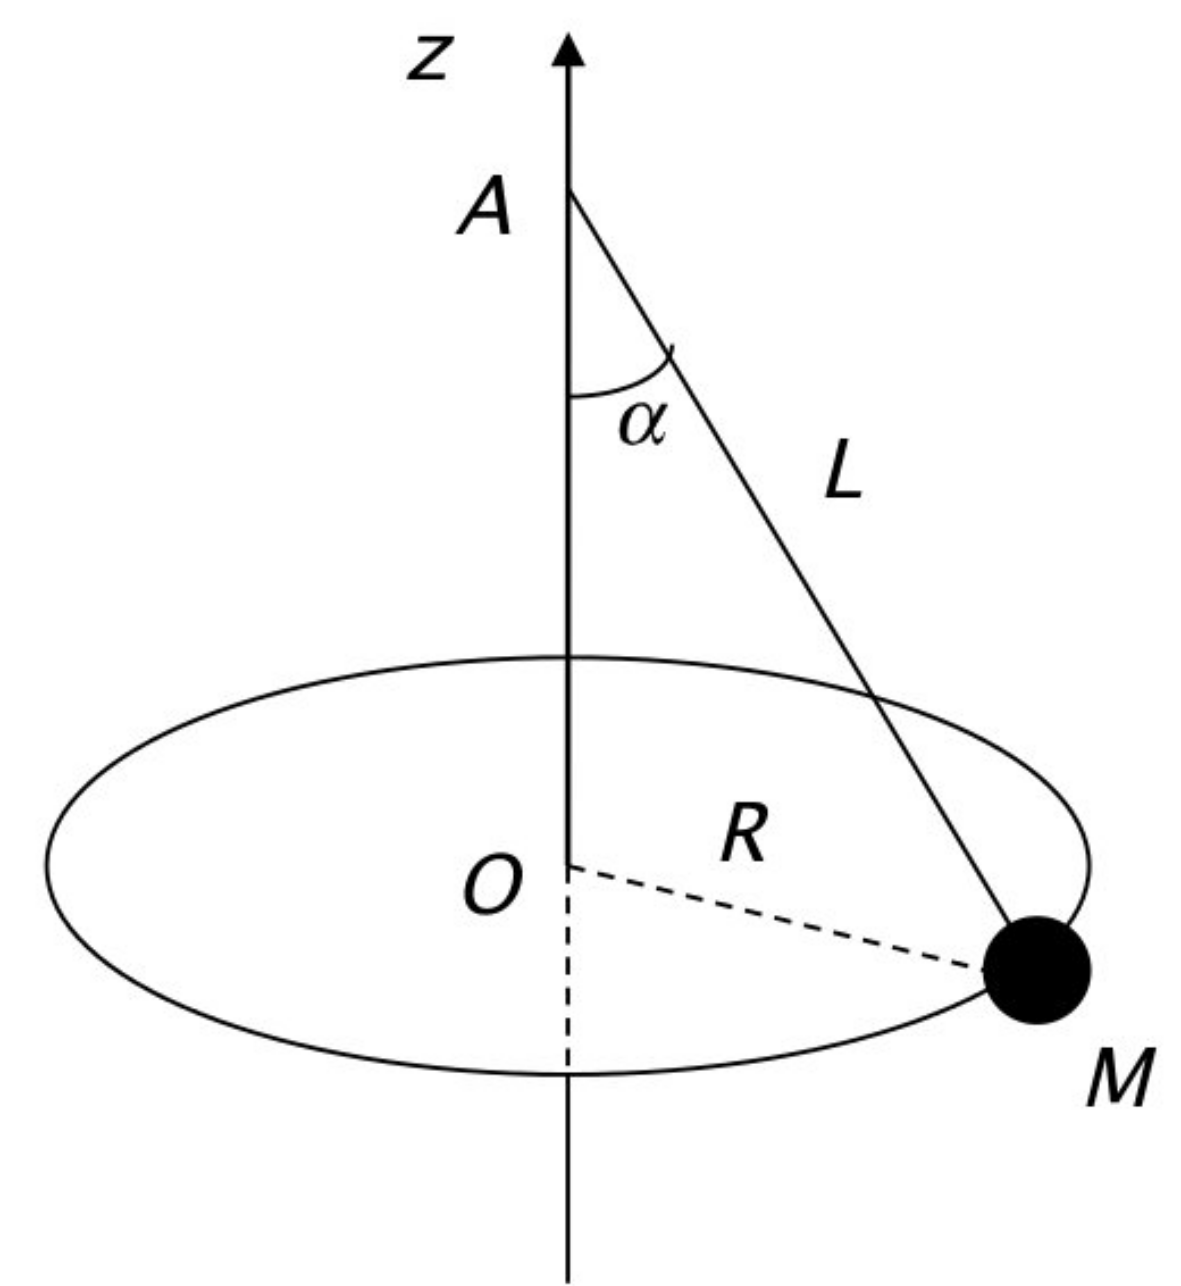
\includegraphics[width=\linewidth]{pendule_conique-plain}
		\end{center}
	\end{minipage}
}%

\QR<[start=2]>{%
	Effectuer un bilan des forces s'appliquant à la masse et les écrire
	dans la base choisie.
}{%
  \leavevmode\vspace*{-15pt}\relax
	\begin{itemize}[label=$\diamond$, leftmargin=10pt]
		\item[b]{Système}~: \{M\} masse $m$
		\item[b]{Référentiel}~: $\Rc\ind{labo}$ supposé galiléen
		\item[b]{Repère}~: $(\Or, \ur, \ut, \uz)$ (voir schéma)
	\end{itemize} \smallbreak
	\begin{minipage}{0.65\linewidth}
		\begin{itemize}[label=$\diamond$, leftmargin=10pt]
			\item[b]{Repérage}~: $R = \cte\Ra\dot{R} = 0$, $\tp = \w =
				\cte\Ra\dot{\w} = 0$~:
			\begin{align*}
				\OM       & = R\ur = L\sin\a\ur \\
				\vf_{\Mr} & = L\tp\sin\a\ut     \\
				          & = L\w\sin\a\ut      \\
				\af_{\Mr} & = -L\w^2\sin\a\ur
			\end{align*}
			\item[b]{BDF}~:
			\[
				\begin{array}{ll}
					\textbf{Poids}   & \Pf = m\gf = -mg\uz             \\
					\textbf{Tension} & \Tf = T(-\sin\a\ur + \cos\a\uz)
				\end{array}
			\]
		\end{itemize}
	\end{minipage}
	\hfill
	\begin{minipage}{0.30\linewidth}
		\begin{center}
			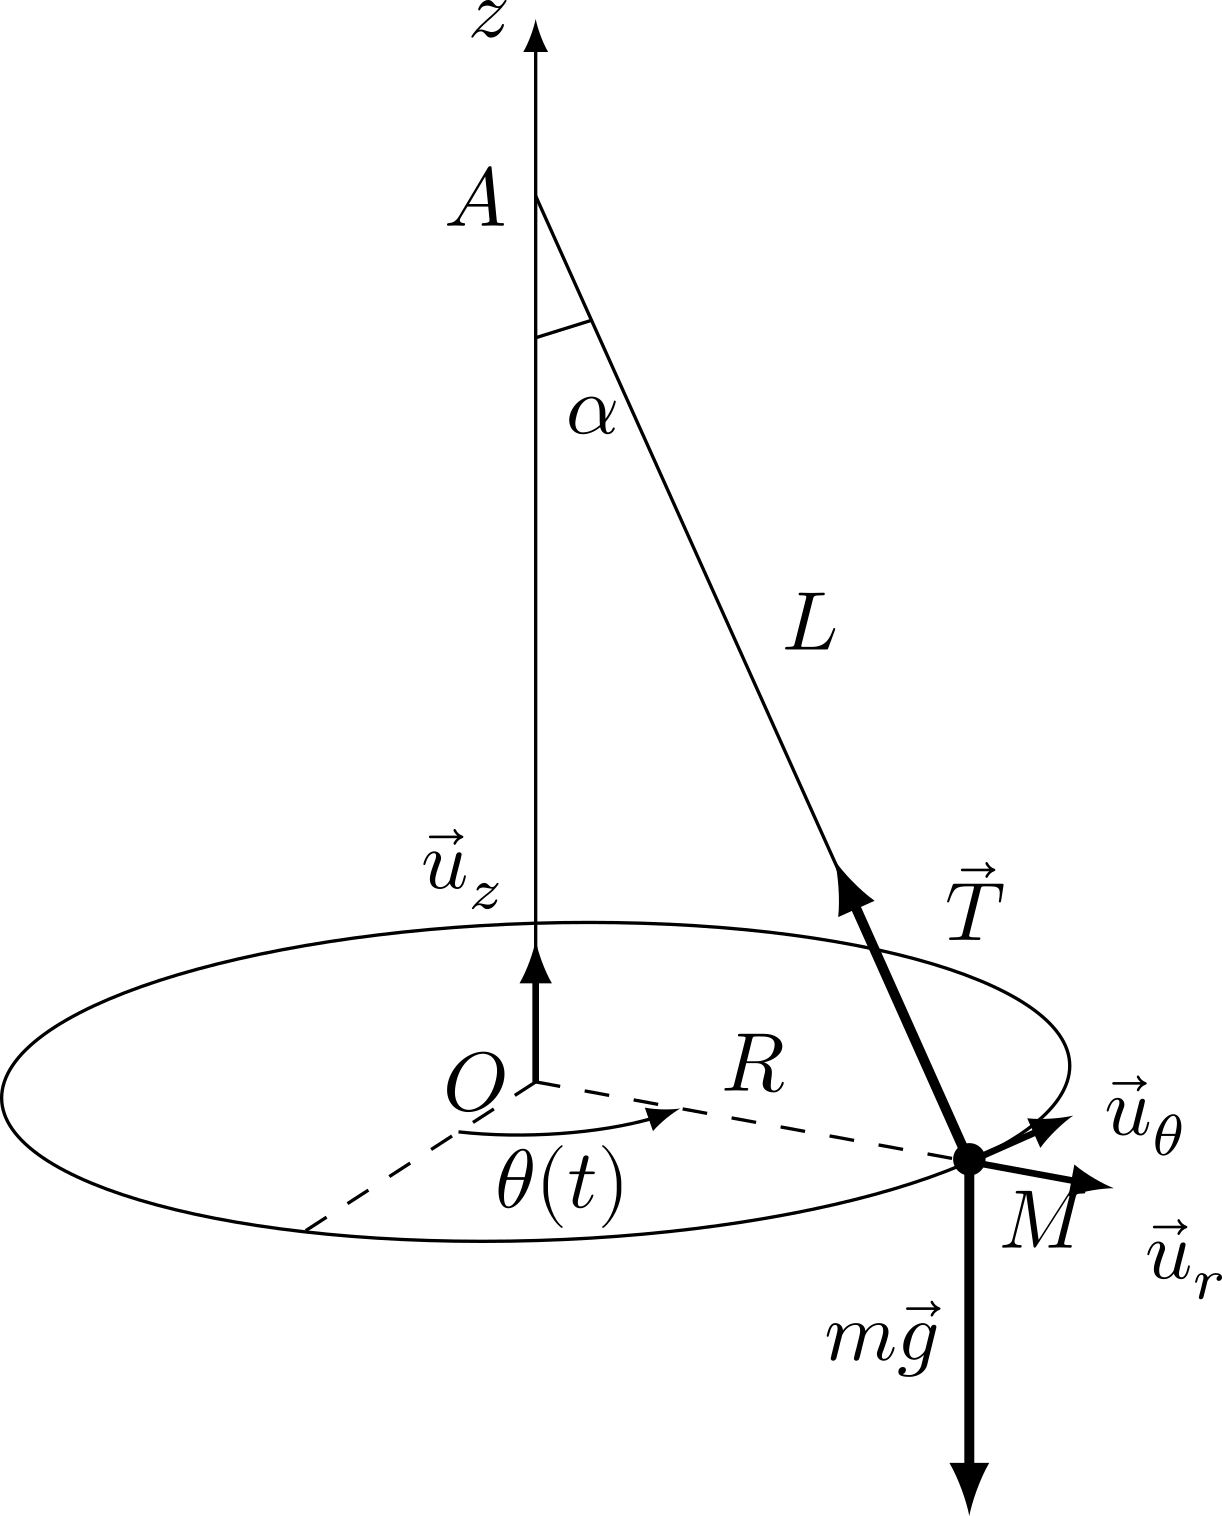
\includegraphics[width=\linewidth]{pendule_corr}
		\end{center}
	\end{minipage}
}
\QR{%
	Appliquer le PFD puis exprimer $\cos\a$ en fonction de $g$, $L$ et
	$\w$. En déduire que la vitesse angulaire doit forcément être supérieure
	à une vitesse angulaire limite $\w_{\lim}$ pour qu'un tel mouvement
	puisse être possible.
}{%
	On applique le PFD~:
	\begin{gather*}
		m\af = \Pf + \Tf
		\Lra
		\left\{
		\begin{aligned}
			-mL\w^2\cancel{\sin\a} & = -T\cancel{\sin\a} \\
			0                      & = T\cos\a -mg
		\end{aligned}
		\right.
		\Lra
		\left\{
		\begin{aligned}
			T & = mL\w^2            \\
			T & = \frac{mg}{\cos\a}
		\end{aligned}
		\right.
		\shortintertext{Soit}
		mL\w^2 = \frac{mg}{\cos\a}
		\Lra
		\boxed{\cos\a = \frac{g}{L\w^2}}
	\end{gather*}
	Pour que ce mouvement soit possible, il faut que $\cos\a < 1$, soit
	\begin{gather*}
		\frac{g}{L\w^2} < 1
		\Lra
		\boxed{\w \geq \sqrt{\frac{g}{L}} = \w_{\lim}}
	\end{gather*}
}
\QR{%
	Que dire du cas où $\w$ devient très grande~?
}{%
	Si $\w \gg \w_{\lim}$, alors $\cos\a \xrightarrow[\w \gg \w_{\lim}]{} 0$
	donc \fbox{$\a\xrightarrow[\w \gg \w_{\lim}]{} \pi/2$}~: le mouvement
	devient simplement circulaire, et se fait dans le plan horizontal
	contenant A.
}
\QR{%
	Application numérique~: calculer $\a$ pour $L = \SI{20}{cm}$ et $\w =
		\SI{3}{tours.s^{-1}}$.
}{%
	\leftcenters{On trouve}{\fbox{$\cos\a = \num{0.138} \Lra \a =
				\ang{82}$}}
}
\end{document}
